\section{Atividades}

Neste módulo, foram realizadas atividades práticas voltadas à exploração de
mecanismos de proteção e monitoramento de segurança em ambientes Windows Server
2022 e Kali Linux. As tarefas envolveram a análise de recursos nativos de
segurança do Windows, incluindo integridade de memória, manutenção automática,
controle de aplicativos, proteção contra exploits e gerenciamento de
atualizações do sistema operacional.

Também foram executadas atividades em ambiente Linux com foco em ferramentas de
segurança defensiva, incluindo a utilização do antivírus ClamAV para varredura
de arquivos e diretórios, além da configuração e execução do sistema de
detecção de intrusão Suricata com regras da comunidade para monitoramento de
eventos de rede e geração de logs de segurança.

\newpage

\question[Atividade 10.1]{Explorando recursos de integridade de memória e manutenção no Windows Server 2022}

\begin{figure}[H]
\centering
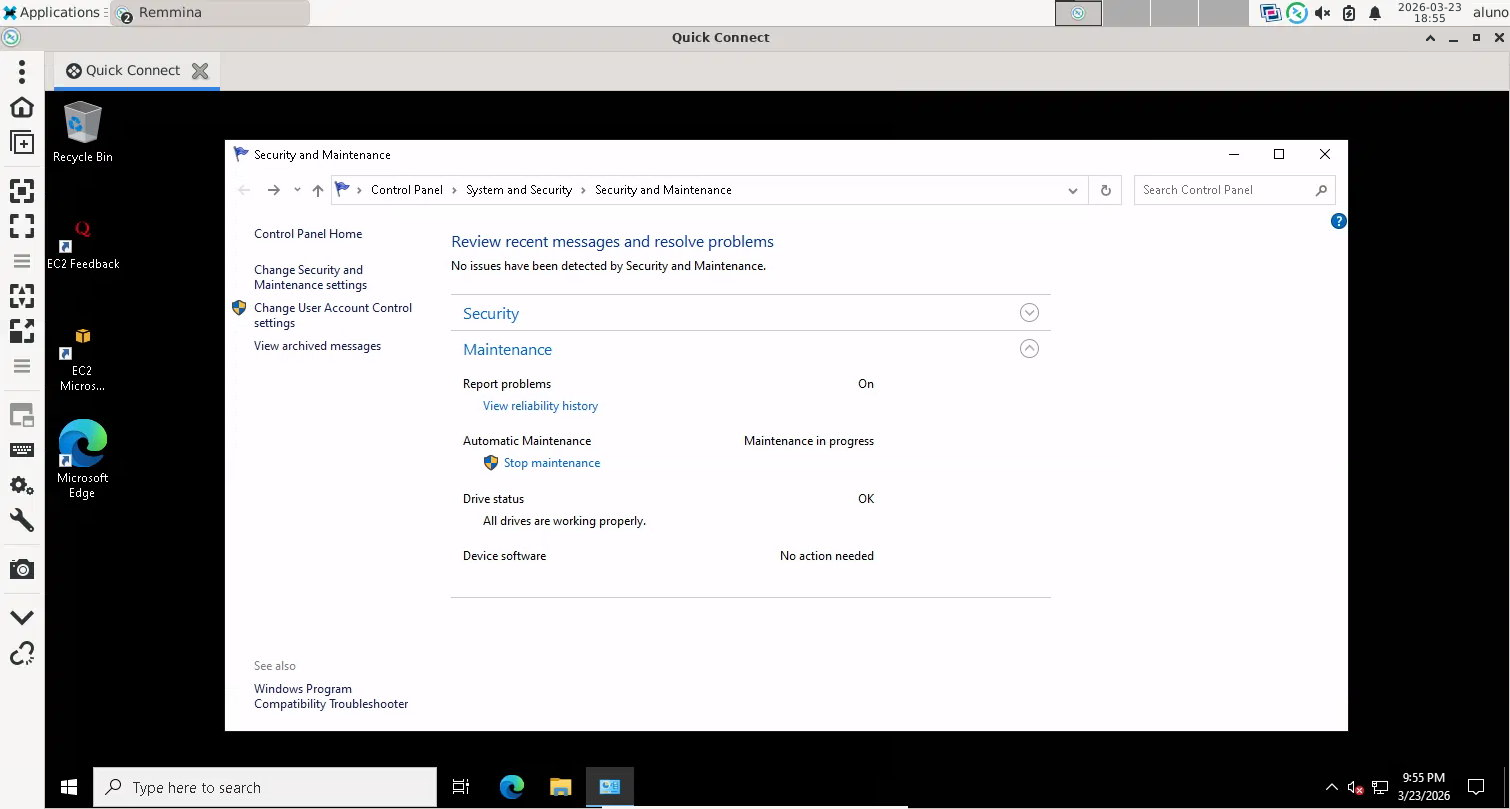
\includegraphics[width=0.99\textwidth]{./fig/fig10.1.png}
\caption{Execução manual da manutenção do sistema com o status ``Maintenance in progress'' no Windows Server 2022}
\label{fig:fig10.1}
\end{figure}

\newpage

\question[Atividade 10.2]{Controle de aplicativos, navegadores e proteções contra exploits}

\begin{figure}[H]
\centering
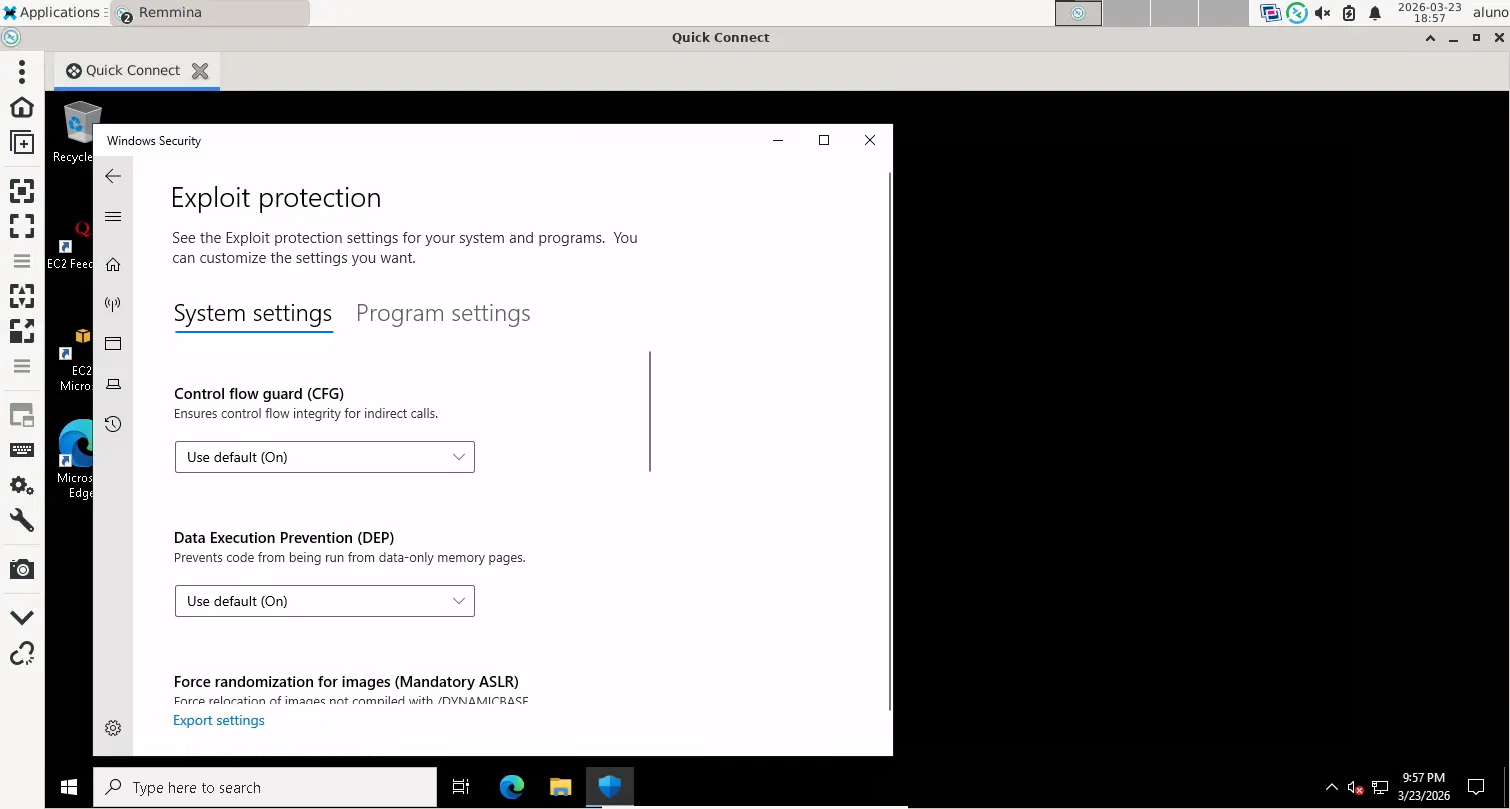
\includegraphics[width=0.99\textwidth]{./fig/fig10.2.png}
\caption{Visualização das proteções avançadas habilitadas em ``Exploit protection settings'' no Windows Security}
\label{fig:fig10.2}
\end{figure}

\newpage

\question[Atividade 10.3]{Gerenciamento de atualizações no Windows Server 2022}

\begin{figure}[H]
\centering
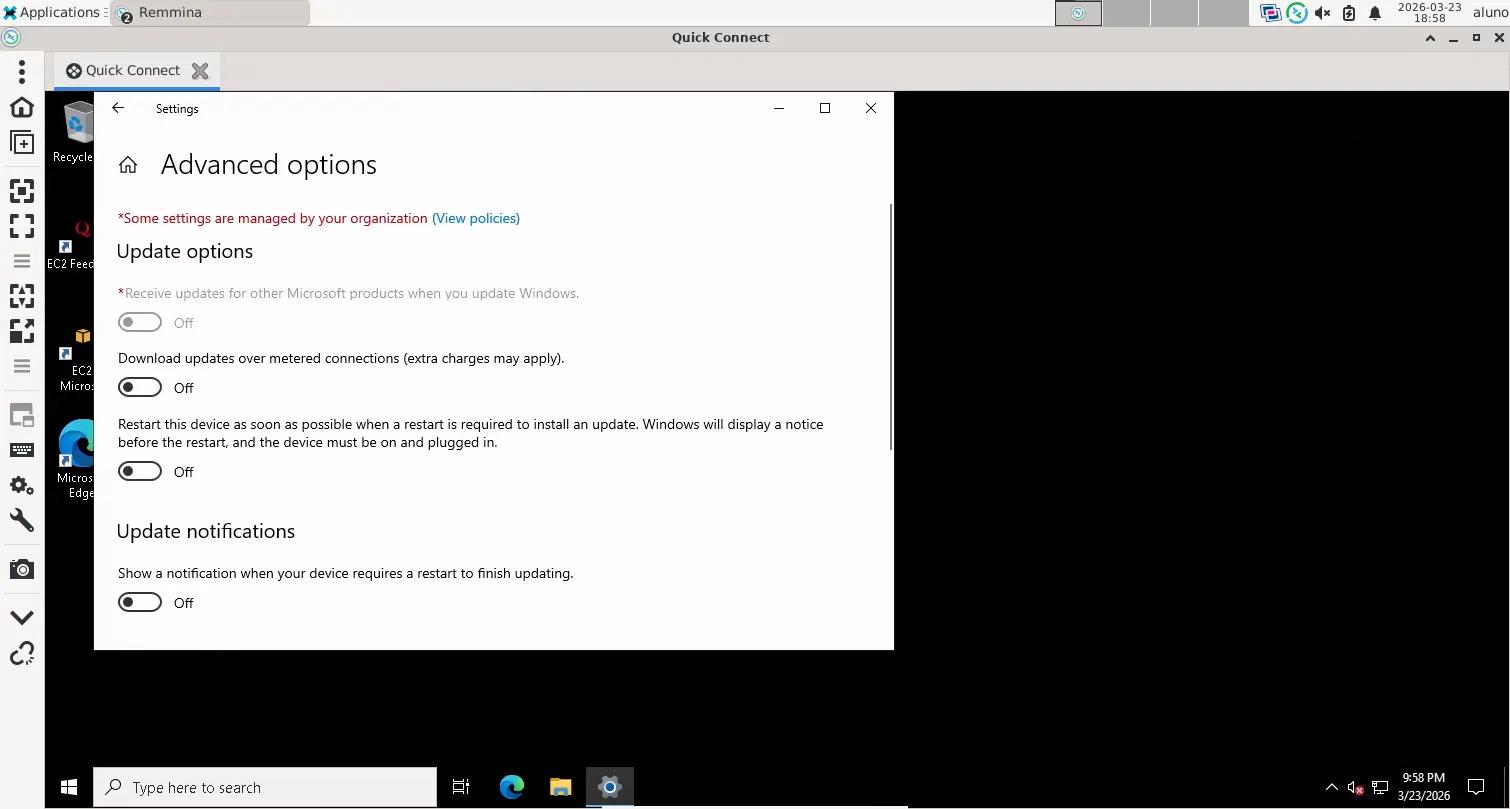
\includegraphics[width=0.99\textwidth]{./fig/fig10.3.png}
\caption{Configuração das opções avançadas de atualização com campos de notificação e atualização habilitados}
\label{fig:fig10.3}
\end{figure}

\newpage

\question[Atividade 10.4]{Escaneamento de arquivos com o antivírus ClamAV no Kali Linux}

\begin{figure}[H]
\centering
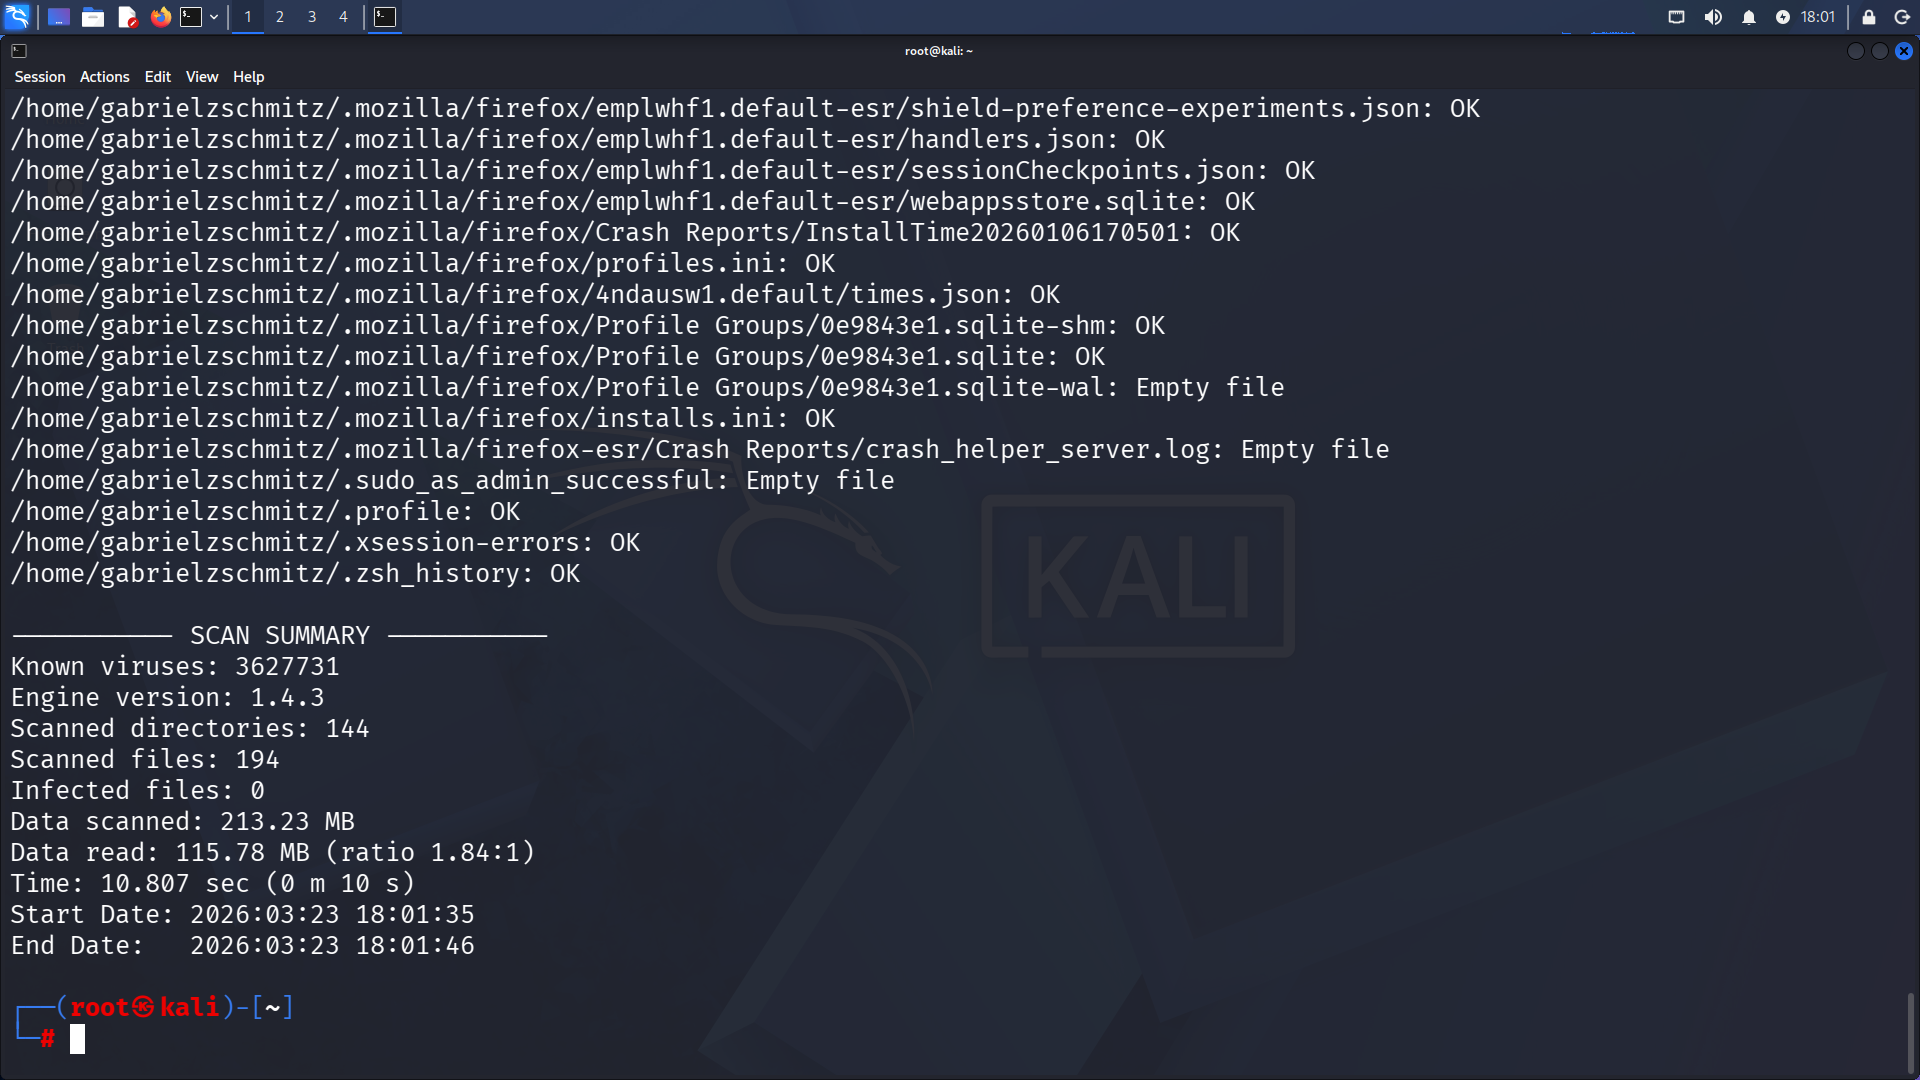
\includegraphics[width=0.99\textwidth]{./fig/fig10.4.png}
\caption{Resumo final do escaneamento recursivo com ClamAV apresentando estatísticas de arquivos analisados}
\label{fig:fig10.4}
\end{figure}

\newpage

\question[Atividade 10.5]{Execução do Suricata HIDS e verificação de logs no Kali Linux}

\begin{figure}[H]
\centering
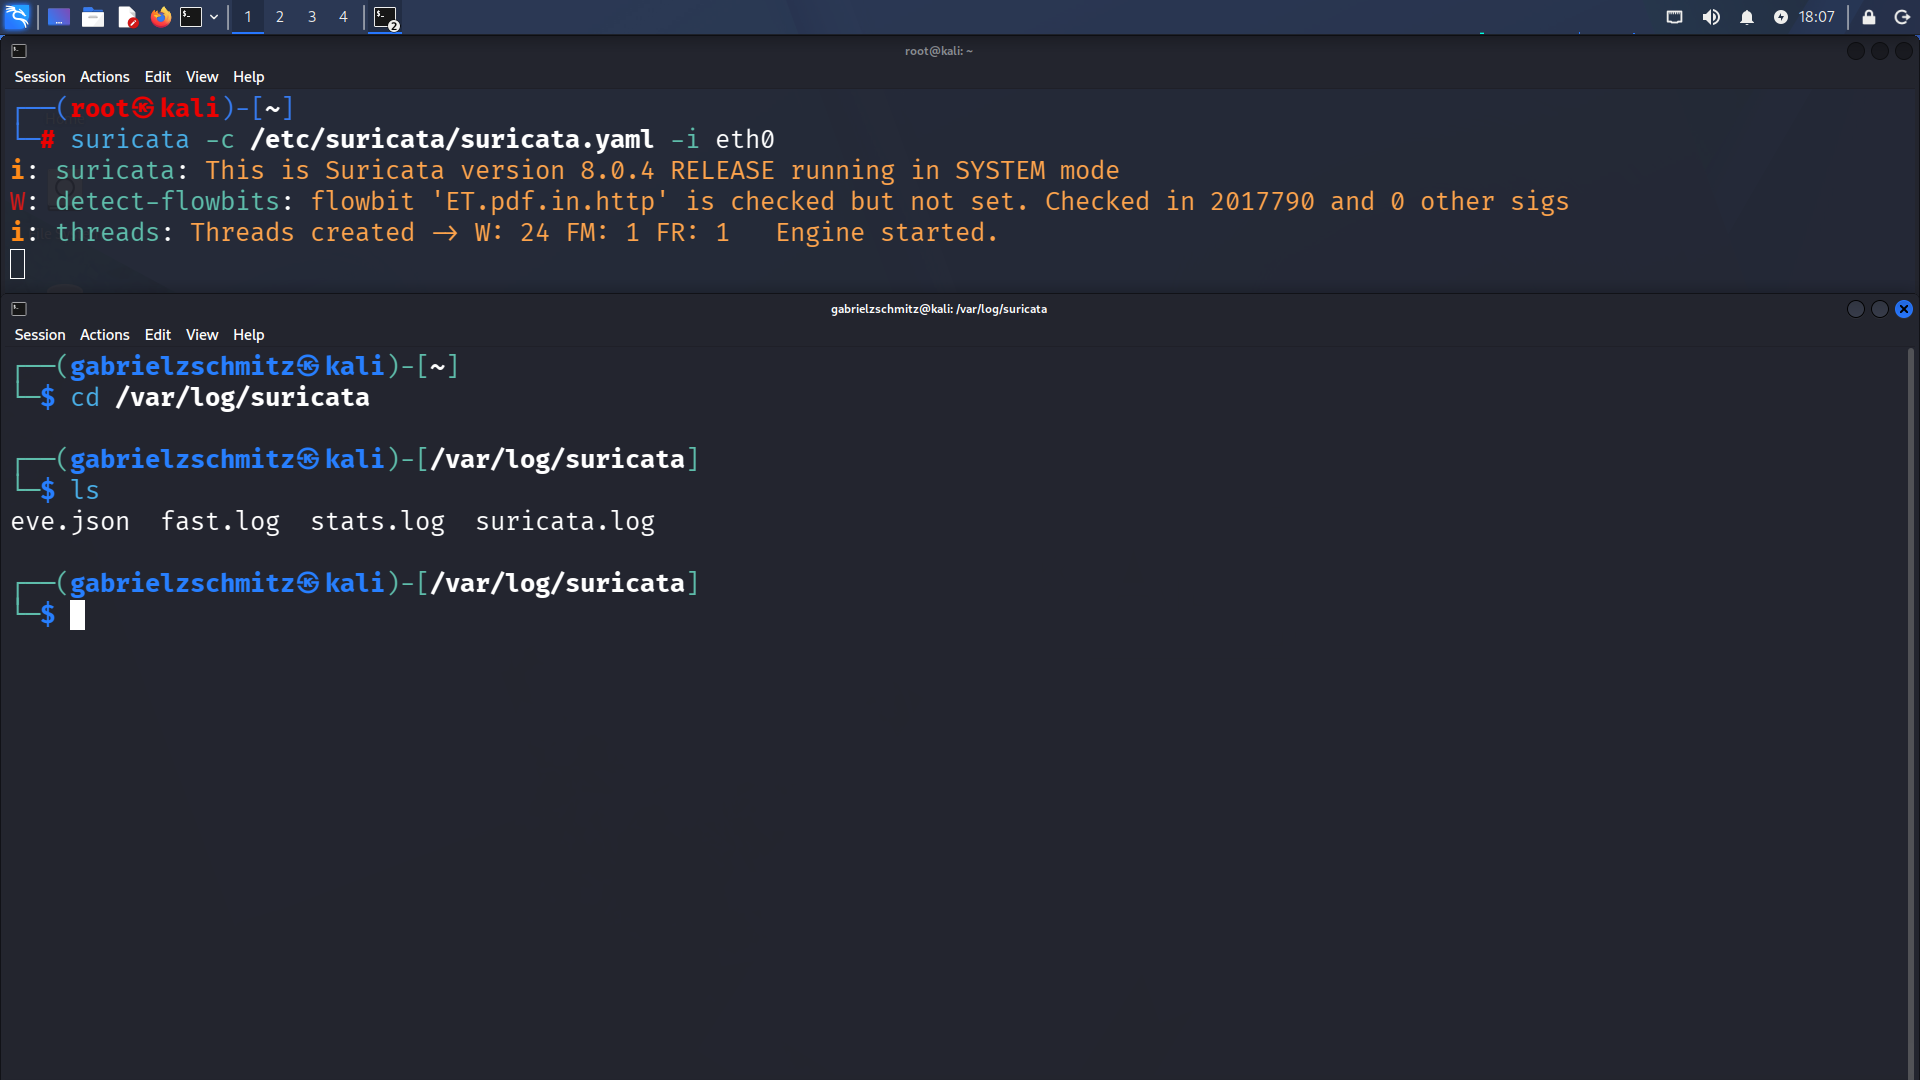
\includegraphics[width=0.99\textwidth]{./fig/fig10.5.png}
\caption{Listagem dos arquivos de log gerados pelo Suricata no diretório /var/log/suricata}
\label{fig:fig10.5}
\end{figure}
